\subsection{Конфигурации планет}
\term{Внутренними планетами} называются планеты, большая полуось орбиты
$a$ которых меньше большой полуоси орбиты Земли $a_\oplus$. Отсюда следует, что для наблюдателя на Земле \imp{внутренними} планетами являются лишь Венера и Меркурий, остальные относятся к \imp{внешним}. Для таких планет выделяют три основные конфигурации: \imp{верхнее соединение}, \imp{нижнее соединение} и \imp{максимальная элонгация}. Различают две максимальные элонгации~--- \term{западную} и \term{восточную}, когда планета наблюдается к западу и к востоку от Солнца соответственно.

Внутренняя планета находится в \term{верхнем соединении}, когда Земля, Солнце и планета лежат на одной прямой, при этом планета и Земля располагаются по разные стороны от Солнца. Если пренебречь наклоном орбит планет к плоскости эклиптики, то для наблюдателя на Земле планета находится точно за Солнцем.

\begin{minipage}{0.36\tw}
	\term{Нижнее соединение} внутренней планеты происходит когда Земля, Солнце и планета, также как и в случае верхнего соединения, располагаются на одной прямой, но для нижнего соединения планета должна находиться между Солнцем и Землей. Если бы орбиты всех планет лежали в одной плоскости, тогда в момент каждого нижнего соединения внутренней планеты наблюдалось бы её прохождение по диску Солнца для наблюдателя на внешней планете.
\end{minipage}
\begin{minipage}{0.63\tw}
	\centering
	\vspace{-1pc}
	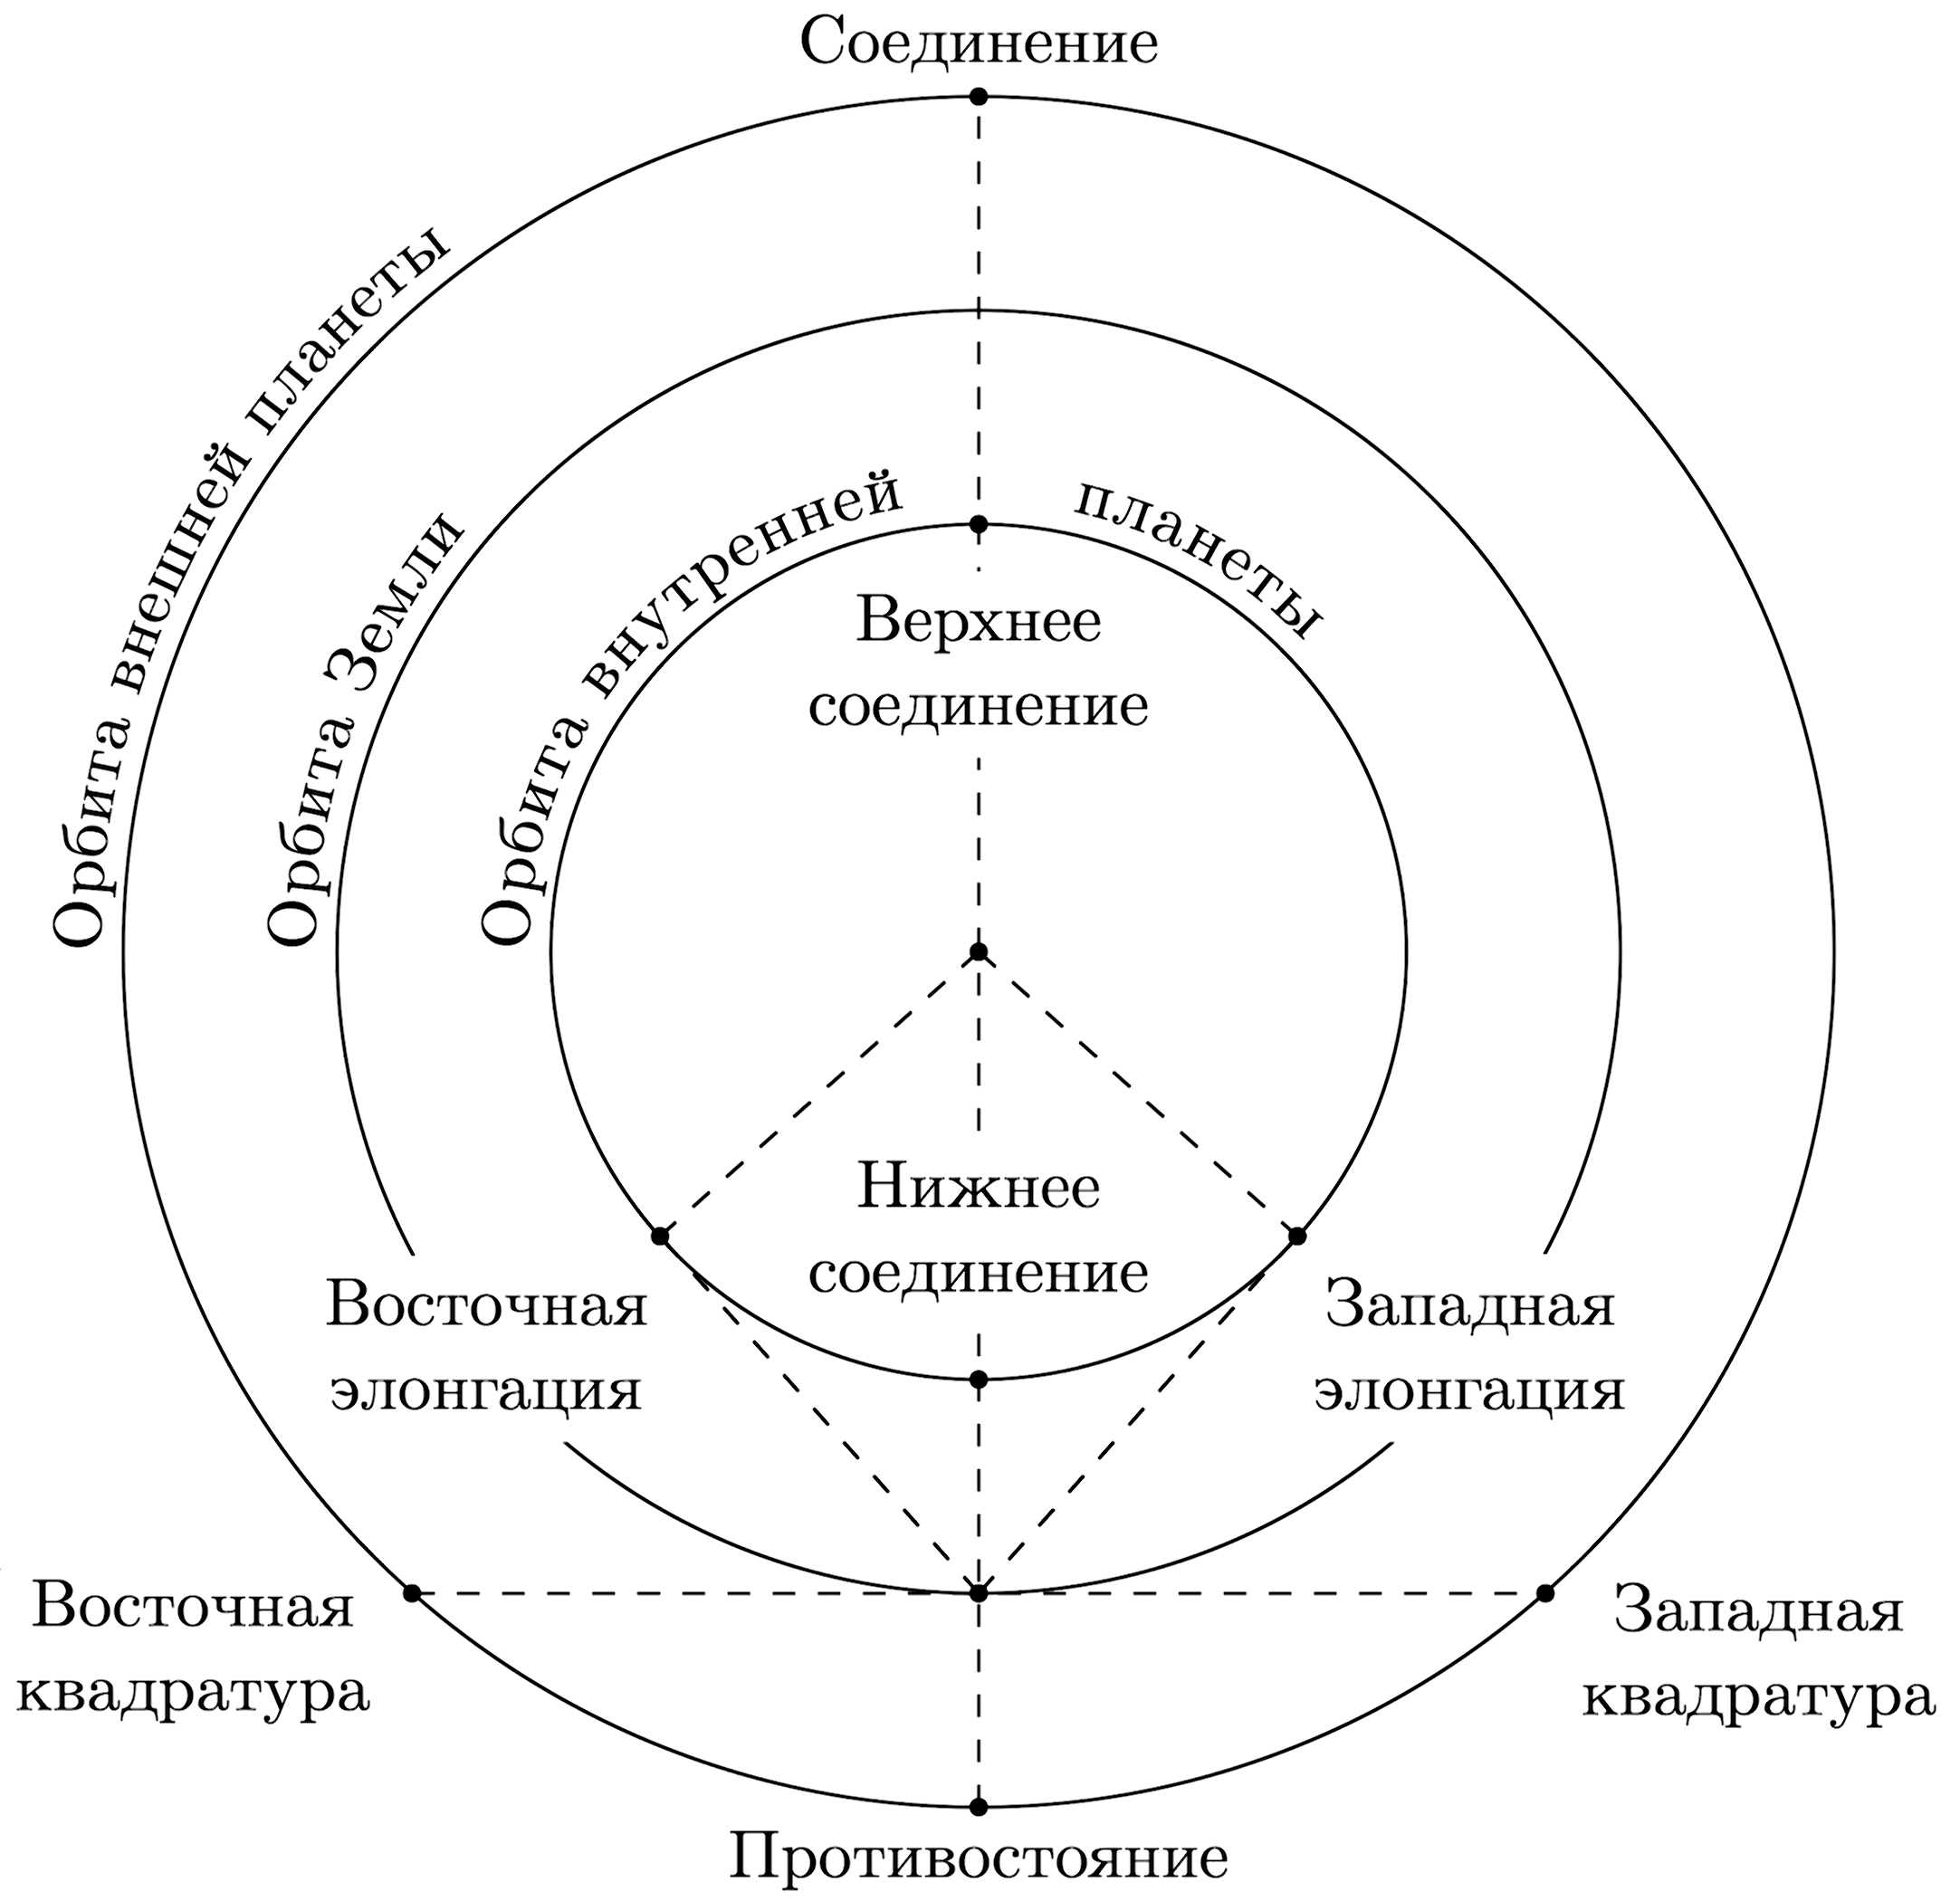
\includegraphics[width=\tw]{planet-config}
	%\scriptsize
	%\begin{tikzpicture}
	%\fill [draw=black, fill=none,
	%         postaction={decorate,decoration={raise=3pt,text along path,
	%           text={Орбита Земли}}}
	%]
	%  (-2.5, 0) arc (180:-180:2.5cm and 2.5cm);
	%
	%\fill [draw=black, fill=none,
	%         postaction={decorate,decoration={raise=3pt,text along path,
	%           text={Орбита внутренней~~~~~~~планеты}}}
	%           ]
	%  (-1.5, 0) arc (180:-180:1.5cm and 1.5cm);
	%
	%\fill [draw=black, fill=none,
	%         postaction={decorate,decoration={raise=3pt,text along path,
	%           text={Орбита внешней планеты}}}
	%           ]
	%  (-3.5, 0) arc (180:-180:3.5cm and 3.5cm);
	%
	%\draw [dashed] (-2.65, -3) -- (2.65, -3);
	%\draw [dashed] (0, -4) -- (0, 4);
	%\draw [dashed] (0, -3) -- (-1.49, -1.33);
	%\draw [dashed] (0, 0) -- (-1.49, -1.33);
	%\draw [dashed] (0, -3) -- (1.49, -1.33);
	%\draw [dashed] (0, 0) -- (1.49, -1.33);
	%
	%\filldraw [black] (0, 0) circle (1pt);
	%\filldraw [black] (-1.49, -1.33) circle (1pt);
	%\filldraw [black] (1.49, -1.33) circle (1pt);
	%\filldraw [black] (2.65, -3) circle (1pt);
	%\filldraw [black] (-2.65, -3) circle (1pt);
	%\filldraw [black] (0, -3) circle (1pt);
	%\filldraw [black] (0, 2) circle (1pt);
	%\filldraw [black] (0, 4) circle (1pt);
	%\filldraw [black] (0, -2) circle (1pt);
	%\filldraw [black] (0, -4) circle (1pt);
	%
	%\draw (-3.7, -3.7) -- (-3.7, -3.7) node  [above,align=center,midway]{Западная\\квадратура};
	%
	%\draw (3.7, -3.7) -- (3.7, -3.7) node  [above,align=center,midway]{Восточная\\квадратура};
	%
	%\draw (0, -4.5) -- (0, -4.5) node  [above,align=center,midway]{Противостояние};
	%
	%\draw (0, 4) -- (0, 4) node  [above,align=center,midway]{Соединение};
	%
	%\draw (0, 0.9) -- (0, 0.9) node  [fill=white,above,align=center,midway]{Верхнее\\соединение};
	%
	%\draw (0, -1.75) -- (0, -1.75) node  [fill=white,above,align=center,midway]{Нижнее\\соединение};
	%
	%\draw (0.6, -3.4) -- (0.6, -3.4) node  [above,align=center,midway]{\ttfamily Земля};
	%
	%\draw (0.7, -0.2) -- (0.7, -0.2) node  [above,align=center,midway]{\ttfamily Солнце};
	%
	%\draw (2.3, -2.3) -- (2.3, -2.3) node  [fill=white,above,align=center,midway]{Западная\\элонгация};
	%
	%\draw (-2.3, -2.3) -- (-2.3, -2.3) node  [fill=white,above,align=center,midway]{Восточная\\элонгация};
	%
	%\end{tikzpicture}
	\captionof{figure}{Конфигурации планет}
\end{minipage}\\

\term{Элонгацией} планеты называется угол Солнце -- Земля -- планета, отсюда очевидно, что \imp{максимальная элонгация} внутренней планеты наблюдается в момент, когда прямая Земля -- планета является касательной к орбите планеты, то есть угол Солнце -- планета -- Земля является прямым.

\term{Внешними планетами} называются планеты, большая полуось орбиты $a$ которых больше большой полуоси орбиты Земли $a_\oplus$. Для таких планет также существуют три основные конфигурации: \imp{соединение}, \imp{противостояние} и \imp{квадратура}. Квадратура бывает \term{западная} и \term{восточная}, в какой именно квадратуре находится внешняя планета определяется аналогично максимальной элонгации.

\term{Соединение} внешней планеты, подобно верхнему соединению внутренней планеты, наблюдается в момент, когда Солнце, Земля и планета находятся на одной прямой, при этом Солнце находится между планетой и Землей. В этот момент для наблюдателя на внешней планете Земля, являясь внутренней планетой, наблюдается в верхнем соединении.

Аналогично, когда планета, Солнце и Земля располагаются на одной прямой, но Солнце и планета лежат по разные стороны от Земли, считается, что внешняя планета находится в \term{противостоянии}. Земля же находится в нижнем соединении для наблюдателя на внешней планете, наблюдаемой в противостоянии.

\term{Квадратурой} называется конфигурация, когда угол между направлениями на планету и Солнце (угол {\slshape Солнце -- Земля -- планета}) является прямым. Стоит заметить, что для наблюдателя на планете Земля будет наблюдаться в максимальной элонгации, причем если планета с Земли наблюдалась в восточной квадратуре, тогда Земля будет в западной максимальной элонгации и наоборот.

